\section{Programación Paralela}

\begin{ejercicio}
    Un programa tarda $\unit[40]{s}$ en ejecutarse en un multiprocesador. Durante un 20\% de ese tiempo se
    ha ejecutado en cuatro procesadores; durante un 60\%, en tres; y durante el 20\% restante, en un procesador
    (consideramos que se ha distribuido la carga de trabajo por igual entre los procesadores que colaboran en la
    ejecución en cada momento, despreciamos sobrecarga).
    \begin{enumerate}
        \item ¿Cuánto tiempo tardaría en ejecutarse el programa
        en un único procesador?
        \item ¿Cuál es la ganancia en velocidad obtenida con respecto al tiempo de ejecución
        secuencial?
        \item ¿Cuál es la ganancia en eficiencia obtenida con respecto al tiempo de ejecución
        secuencial?
    \end{enumerate}

    Por el enunciado, tenemos que $T_P=\unit[40]{s}$ y $T_O(p)=\unit[0]{s}$. Por tanto:
        \begin{equation*}
            T_P(p) = T_C(p) + \cancelto{0}{T_O(p)} = T_C(p)
        \end{equation*}
    \begin{enumerate}
        \item
        Gracias al enunciado, deducimos que durante $0.2T_P$ se usan 4 procesadores,
        durante $0.6T_P$ se usan 3 y durante $0.2T_P$ se usa un único procesador.
        Por tanto, si ejecutásemos el programa en un único procesador, tendríamos
        que ejecutar de forma secuencial el código correspondiente a los 4 procesadores, luego a los tres procesadores y por último la parte que no es paralelizable.
        Por tanto, tenemos que:
        \begin{equation*}
            T_S = 4\cdot 0.2T_P + 3\cdot 0.6T_P + 0.2T_P = 2.8T_P = 2.8 \cdot \unit[40]{s} = \unit[112]{s}
        \end{equation*}

        \item Calculamos la ganancia:
        \begin{equation*}
            S(4) = \dfrac{T_S}{T_P(4)} = \dfrac{2.8\cancel{T_P}}{\cancel{T_P}} = 2.8 
        \end{equation*}

        \begin{observacion}
            Buscamos ahora comprobar si la ganancia obtenida es correcta.
            Suponiendo que podemos paralelizar todo el programa, el tiempo paralelo será $T_P(p) = \nicefrac{T_S}{p}$.
            Por otro lado, si no podemos paralelizar nada, el tiempo paralelo será $T_P(p) = T_S$. Por tanto, tenemos que $\nicefrac{T_S}{p}\leq T_P(p) \leq T_S$.
            Por tanto:
            \begin{equation*}
                1 = \dfrac{T_S}{T_S} \leq \dfrac{T_S}{T_P(p)} = S(p) \leq \dfrac{T_S}{\nicefrac{T_S}{p}} = p
            \end{equation*}
            Al ser $1 < 2.8 < 4$, podemos intuir que hemos calculado bien la solución.
        \end{observacion}

        \item
        Calculamos la eficiencia:
        \begin{equation*}
            E(p) = \dfrac{\text{Prestaciones}(p)}{p\cdot \text{Prestaciones}(1)} = \dfrac{S(p)}{p} = \dfrac{2.8}{4} = 0.7
        \end{equation*}

        \begin{observacion}
            Buscamos ahora comprobar si la eficiencia obtenida es correcta.
            Como $1\leq S(p)\leq p$, tenemos que:
            \begin{equation*}
                \dfrac{1}{p} \leq \dfrac{S(p)}{p} = E(p) \leq 1
            \end{equation*}
            Al ser $0.25=\nicefrac{1}{4} \leq 0.7 \leq 1$, podemos intuir que hemos calculado bien la solución.
        \end{observacion}
        
    \end{enumerate}
\end{ejercicio}

\begin{ejercicio}
    Un programa tarda $\unit[40]{s}$ en ejecutarse en un procesador $P_1$, y requiere $\unit[30]{s}$ en otro procesador
    $P_2$. Si se dispone de los dos procesadores para la ejecución del programa (despreciamos sobrecarga):
    \begin{enumerate}
        \item ¿Qué tiempo tarda en ejecutarse el programa si la carga de trabajo se distribuye por igual entre los
        procesadores $P_1$ y $P_2$?
        \item ¿Qué distribución de carga entre los dos procesadores $P_1$ y $P_2$ permite el menor tiempo de
        ejecución utilizando los dos procesadores en paralelo? ¿Cuál es este tiempo?
    \end{enumerate}


    Del enunciado, tenemos que $T_S^{P_1} = \unit[40]{s}$, $T_S^{P_2} = \unit[30]{s}$ y $T_O(p) = 0$. Por tanto:
    \begin{equation*}
        T_P(p) = T_C(p) + \cancelto{0}{T_O(p)} = T_C(p)
    \end{equation*}

    \begin{enumerate}
        \item 
            Si a los dos le asignamos la mitad del trabajo, tendremos que:
            \begin{equation*}
                T_S^{P_1}\left(\frac{1}{2}\right) = \frac{1}{2}\cdot \unit[20]{s} = \unit[10]{s} \quad \quad T_S^{P_2}\left(\frac{1}{2}\right) = \frac{1}{2}\cdot \unit[30]{s} = \unit[15]{s}
            \end{equation*}
            
            Por tanto:
            \begin{equation*}
                T_P^{P_1, P_2}\left(\frac{1}{2}, \frac{1}{2}\right) = \max\left\{T_S^{P_1}\left(\frac{1}{2}\right), T_S^{P_2}\left(\frac{1}{2}\right)\right\} = \max\{\unit[10]{s}, \unit[15]{s}\} = \unit[15]{s}
            \end{equation*}

            Como inconveniente, tenemos que el procesador $P_1$ está ocioso durante 5 segundos, por lo que no es la mejor solución.

        \item 
        Repartimos el trabajo de forma que a $P_1$ le asignamos una fracción de trabajo de $x$, por lo que a $P_2$ le tendremos que asignar una carga de $1-x$. Para obtener los mejores tiempos, imponemos que:
        \begin{equation*}
            T_S^{P_1}(x) = T_S^{P_2}(1-x) \Longleftrightarrow
            x\cdot \unit[20]{s} = (1-x)\cdot \unit[30]{s} \Longleftrightarrow
            2x = 3-3x \Longleftrightarrow x = \frac{3}{5}
        \end{equation*}

        Por tanto, tenemos que $T_S^{P_1}\left(\nicefrac{3}{5}\right) = T_S^{P_2}\left(\nicefrac{2}{5}\right) = \nicefrac{3}{5}\cdot \unit[20]{s} = \unit[12]{s}$. 
        Por tanto, el tiempo de ejecución en paralelo será de:
        \begin{equation*}
            T_P^{P_1, P_2}\left(\nicefrac{3}{5}, \nicefrac{2}{5}\right) = \max\left\{T_S^{P_1}\left(\nicefrac{3}{5}\right), T_S^{P_2}\left(\nicefrac{2}{5}\right)\right\} = \max\{\unit[12]{s}, \unit[12]{s}\} = \unit[12]{s}
        \end{equation*}

        Como vemos, al realizar una distribución de carga equilibrada obtenemos un tiempo de ejecución menor.
    \end{enumerate}

    

\end{ejercicio}

\begin{ejercicio}
    ¿Cuál es fracción de código paralelo de un programa secuencial que, ejecutado en paralelo en 8
    procesadores, tarda un tiempo de $\unit[100]{ns}$, durante $\unit[50]{ns}$ utiliza un único procesador y durante otros $\unit[50]{ns}$
    utiliza 8 procesadores (distribuyendo la carga de trabajo por igual entre los procesadores)?\\

    En primer lugar, cabe destacar que vamos a suponer que el tiempo de sobrecarga es despreciable, ya que si no no podríamos dar ninguna solución.
    Sabiendo esto, tenemos que el tiempo secuencial sería:
    \begin{equation*}
        T_S = 1\cdot \unit[50]{ns} + 8\cdot \unit[50]{ns} = 9\cdot \unit[50]{ns} 
    \end{equation*}

    El tiempo secuencial que tardaría en ejecutarse la parte paralelizada (código paralelo)
    sería $8\cdot \unit[50]{ns}$. por tanto, tenemos que la fracción del código que es paralelizable es:
    \begin{equation*}
        \frac{8\cdot \unit[50]{ns}}{9\cdot \unit[50]{ns}} = \frac{8}{9}
    \end{equation*}
    Por tanto, la fracción de código paralelo es de $\nicefrac{8}{9}$.
\end{ejercicio}

\begin{ejercicio}
    Un 25\% de un programa no se puede paralelizar, el resto se puede distribuir por igual entre
    cualquier número de procesadores. ¿Cuál es el máximo valor de ganancia de velocidad que se podría
    conseguir al paralelizarlo en $p$ procesadores, y con infinitos? ¿A partir de cuál número de procesadores se
    podrían conseguir ganancias mayores o iguales que 2?\\

    El máximo valor de ganancia que podemos obtener resulta cuando el tiempo de sobrecarga es despreciable:
    \begin{equation*}
        T_P(p) = T_C(p) + \cancelto{0}{T_O(p)}
    \end{equation*}

    Una vez sabiendo esto, podemos aplicar la Ley de Amdahl. Dado que un 25\% del programa no puede paralelizarse, tenemos que $f=\nicefrac{1}{4}$. Por tanto, usando dicha Ley tenemos:
    \begin{equation*}
        S(p) \leq \dfrac{1}{f+\dfrac{1-f}{p}} = \dfrac{1}{\dfrac{1}{4}+\dfrac{3}{4p}} = \dfrac{4p}{p+3}
    \end{equation*}
    Esta la mayor ganancia que podemos obtener al paralelizarlo en $p$ procesadores. Tomando límite con $p\to \infty$, tenemos:
    \begin{equation*}
        S_{\max} = \lim_{p\to\infty}S(p) = \lim_{p\to\infty}\dfrac{4p}{p+3} = 4
    \end{equation*}
    Finalmente, nos preguntamos por el número $p$ de procesadores necesarios para conseguir ganancias mayores o iguales que 2:
    \begin{equation*}
        S(p) = \dfrac{4p}{p+3} \geq 2 \Longleftrightarrow 4p\geq 2p+6\Longleftrightarrow 2p\geq 6 \Longleftrightarrow p\geq 3
    \end{equation*}
    Por tanto, necesitamos como mínimo 3 procesadores para obtener una ganancia mayor o igual a $2$.
\end{ejercicio}

\begin{ejercicio}\label{ej:2.5}
    
    En la Figura~\ref{fig:Grafo_2.5}, se presenta el grafo de dependencia entre tareas para una aplicación.
    La figura muestra la fracción del tiempo de ejecución secuencial que la aplicación tarda en ejecutar grupos de tareas del grafo.
    Suponiendo un tiempo de ejecución secuencial de $\unit[60]{s}$, que las tareas no se pueden dividir en tareas de menor granularidad y
    que el tiempo de comunicación es desprecible, obtener el tiempo de ejecución en paralelo y la ganancia en velocidad en un computador con:
    \begin{enumerate}
        \item $4$ procesadores.
        \item $2$ procesadores.
    \end{enumerate}
    \begin{figure}[H]
        \centering
        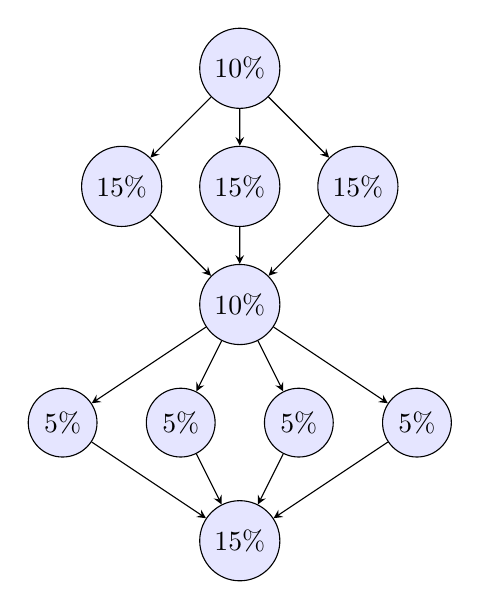
\begin{tikzpicture}[
            every node/.style={circle, draw, fill=blue!10},
            level 1/.style={sibling distance=1.5cm},
            level 2/.style={sibling distance=1cm},
            level 3/.style={sibling distance=1cm},
            level 4/.style={sibling distance=1cm},
            level distance=1.5cm,
            sibling distance=2.5cm,
            edge from parent/.style={draw,-stealth}
            ]
            \node (topnode) at (0,5) {10\%} 
            child{node{15\%}}
            child{node{15\%}}
            child{node{15\%}}
            ;
    
            \node (middlenode) at (0,2) {10\%}
            child{node{5\%}}
            child{node{5\%}}
            child{node{5\%}}
            child{node{5\%}}
            ;
    
            \node(bottomnode) at (0,-1) {15\%};
    
            \foreach \x in {1,2,3,4}{
                \draw[-stealth] (middlenode-\x) -- (bottomnode);
            }
    
            \foreach \x in {1,2,3}{
                \draw[-stealth] (topnode-\x) -- (middlenode);
            }
        \end{tikzpicture}
        \caption{Grafo de tareas del Ejercicio~\ref{ej:2.5}.}
        \label{fig:Grafo_2.5}
    \end{figure}

    Del enunciado, tenemos que $T_S = \unit[60]{s}$ y $T_O(p) = 0$. Por tanto:
    \begin{equation*}
        T_P(p) = T_C(p) + \cancelto{0}{T_O(p)} = T_C(p)
    \end{equation*}
    
    Numeramos las tareas (los nodos) de arriba a abajo y de izquierda a derecha. 
    Observando el gráfico, vemos que el número máximo de nodos en el mismo nivel es 4, luego el número máximo de procesadores (cores) que demos usar será de 4.

    \begin{enumerate}
        \item En este caso, usaremos 4 procesadores, por lo que estamos en el caso ideal como hemos mencionado. Tenemos que:
            \begin{itemize}
                \item La tarea 1 tendrá un tiempo de ejecución de $0.1T_S$.
                \item Las tareas 2, 3 y 4 tendrán tiempos de ejecución $0.15T_S$.
                \item La tarea 5 tendrá un tiempo de ejecución de $0.1T_S$.
                \item Las tareas 6, 7, 8 y 9 tendrán tiempos de ejecución $0.05T_S$.
                \item La tarea 10 tendrá un tiempo de ejecución de $0.15T_S$.
            \end{itemize}

            Además, tenemos que no se pueden ejecutar las tareas de nivel $i+1$ si no se han terminado las del nivel $i$,
            ya que las del siguiente nivel necesitan de los datos generador por el nivel anterior. Por tanto, tenemos que:
            \begin{equation*}
                T_P(4) = 0.1T_S + 0.15T_S + 0.1T_S + 0.05T_S + 0.15T_S = 0.55T_S = 0.55\cdot \unit[60]{s} = \unit[33]{s}
            \end{equation*}

            Calculamos la ganancia:
            \begin{equation*}
                S(4) = \dfrac{T_S}{T_P(4)} = \dfrac{\cancel{T_S}}{0.55\cancel{T_S}} = \dfrac{1}{0.55} = \dfrac{20}{11} \approx 1.82
            \end{equation*}
            Este resultado tiene sentido, ya que $1\leq S(4)\leq p=4$, por lo que la ganacia calculada está dentro del valor mínimo y máximo de esta.
        
        \item En este caso, usaremos 2 procesadores:
            \begin{itemize}
                \item La tarea 1 tendrá un tiempo de ejecución de $0.1T_S$, al igual que en el caso de paradores.
                \item Las tareas 2, 3 y 4 no pueden ejecutarse en paralelo todas a la vez. Tendremos que ejecutar en primer lugar la 2 y la 3 ($0.15T_S$) y después la 4 ($0.15T_S$).
                \item La tarea 5 tendrá un tiempo de ejecución de $0.10T_S$.
                \item Las tareas 6, 7, 8 y 9 no pueden ejecutarse en paralelo todas a la vez. Tendremos que ejecutar en primer lugar la 6 y la 7 ($0.05T_S$) y después la 8 y 9 ($0.05T_S$).
                \item La tarea 10 tendrá un tiempo de ejecución de $0.15T_S$.
            \end{itemize}

            Por tanto, tenemos que:
            \begin{equation*}
                T_P(2) = 0.1T_S + 2\cdot 0.15T_S + 0.1T_S + 2\cdot 0.05 T_S + 0.15 T_S = 0.75 \cdot T_S = \unit[45]{s}
            \end{equation*}

            Como vemos, el tiempo es mayor debido a que los niveles 2 y 4 no los podemos paralelizar de forma completa.
            La ganancia queda:
            \begin{equation*}
                S(2) = \dfrac{T_S}{T_P(2)} = \dfrac{\cancel{T_S}}{0.75\cdot \cancel{T_S}} = \frac{1}{0.75} = \frac{4}{3} \approx 1.333 < 2
            \end{equation*}
    \end{enumerate}
\end{ejercicio}


\begin{ejercicio} \label{ej:2.6}
    Un programa se ha conseguido dividir en 10 tareas. El orden de precedencia entre las tareas se
    muestra con el grafo dirigido de la Figura~\ref{fig:Grafo_2.6}. La ejecución de estas tareas en un procesador supone un tiempo de $\unit[2]{s}$.
    El 10\% de ese tiempo es debido a la ejecución de la tarea 1; el 15\% a la ejecución de la tarea 2; otro 15\% a la ejecución de 3;
    cada tarea 4, 5, 6 o 7 supone el 9\%; un 8\% supone la tarea 8; la tarea 9 un 10\%; por último, la tarea 10 supone un 6\%.
    Se dispone de una arquitectura con 8 procesadores para ejecutar la aplicación. Consideramos que el tiempo de comunicación se puede despreciar.
    \begin{enumerate}
        \item ¿Qué tiempo tarda en ejecutarse el programa en paralelo?
        \item ¿Qué ganancia en velocidad se obtiene con respecto a su ejecución secuencial?
    \end{enumerate}
    \begin{figure}[H]
        \centering
        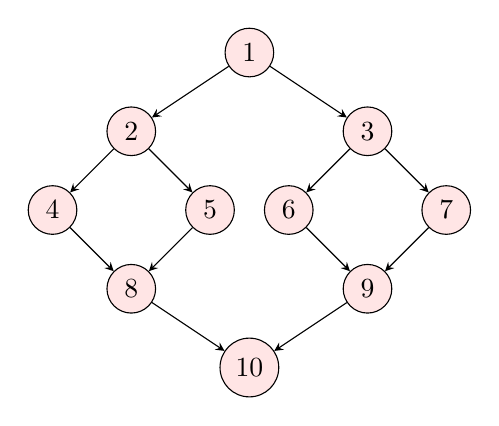
\begin{tikzpicture}[
            every node/.style={circle, draw, fill=red!10},
            level 1/.style={sibling distance=3cm},
            level 2/.style={sibling distance=2cm},
            level 3/.style={sibling distance=2.5cm},
            level 4/.style={sibling distance=1cm},
            level distance=1cm,
            sibling distance=3cm,
            edge from parent/.style={draw,-stealth}]

            \node (topnode) at (0,4) {1} 
                child { node {2}
                    child { node {4}}
                    child { node {5}}
                }
                child { node {3}
                    child { node {6}}
                    child { node {7}}
                }
            ;

            \node(bottomnode) at (0,0) {10} [grow=up]
                child[edge from parent/.style={draw,stealth-}] { node {9}}
                child[edge from parent/.style={draw,stealth-}] { node {8}}
            ;

            \foreach \i in {1,2}{
                \draw[-stealth] (topnode-1-\i) -- (bottomnode-2);
            }

            \foreach \i in {1,2}{
                \draw[-stealth] (topnode-2-\i) -- (bottomnode-1);
            }
        \end{tikzpicture}
        \caption{Grafo de tareas del Ejercicio~\ref{ej:2.6}}
        \label{fig:Grafo_2.6}
    \end{figure}

    Según el grafo~\ref{fig:Grafo_2.6}, como máximo tenemos un total de 4 tareas independientes a ejecutar. Por tanto, a pesar de disponer de 8 procesadores, sólo usaremos 4.

    \begin{enumerate}
        \item Dados los porcentajes del enunciado, calculamos el tiempo de ejecución paralelo a partir del secuencial.
            \begin{align*}
                T_P(4) &= 0.1T_S + 0.15T_S + 0.09T_S + \max\{0.08, 0.1\}T_S + 0.06T_S \\
                       &= 0.5T_S = 0.5\cdot \unit[2]{s} = \unit[1]{s}
            \end{align*}

            Además, como $4$ es el número máximo de procesadores que emplearemos, tenemos que
            $T_P(n) = T_P(4)$ para todo $n\geq 4$, y en particular para $n=8$.
        \item La ganancia respecto a la secuencial es:
            \begin{equation*}
                S(4) = \dfrac{T_S}{T_P(4)} = \dfrac{\unit[2]{s}}{\unit[1]{s}} = 2
            \end{equation*}
            Al igual que ocurría con el tiempo de ejecución en paralelo, para la ganancia tenemos que
            $S(n) = S(4)$ para todo $n\geq 4$, y en particular para $n=8$.
    \end{enumerate}

\end{ejercicio}

\begin{ejercicio}
    Se quiere paralelizar el siguiente trozo de código:
    \begin{minted}[xleftmargin=3cm]{c++}
//  {Cálculos antes del bucle}
for( i=0; i<w; i++) {
    // Código para i
}
// {cálculos después del bucle}
    \end{minted}
    Los cálculos antes y después del bucle suponen un tiempo de $t_1$ y $t_2$, respectivamente.
    Una iteración del ciclo supone un tiempo $t_i$. En la ejecución paralela, la inicialización de $p$ procesos supone un tiempo
    $k_1p$ ($k_1$ constante), los procesos se comunican y se sincronizan, lo que supone un tiempo $k_2p$ ($k_2$ constante); $k_1p+k_2p$
    constituyen la sobrecarga.
    \begin{enumerate}
        \item Obtener una expresión para el tiempo de ejecución paralela del trozo de código en $p$ procesadores ($T_P$).
        \item Obtener una expresión para la ganancia en velocidad de la ejecución paralela con respecto a una ejecución secuencial ($S(p)$).
        \item ¿Tiene el tiempo $T_P$ con respecto a $p$ una característica lineal o puede presentar algún mínimo? ¿Por qué? En caso de presentar un mínimo, ¿para qué número de procesadores $p$ se alcanza?
    \end{enumerate}

    \begin{enumerate}
        \item Para obtener una expresión del tiempo de ejecución en paralelo del trozo de código en $p$ procesadores, necesitamos:
            \begin{equation*}
                T_P(p) = T_C(p) + T_O(p)
            \end{equation*}
            Sabemos ya que $T_O(p) = p(k_1 + k_2)$, pero no tenemos de forma directa $T_C(p)$.
            Tenemos una sección de código no paralelizable (los cálculos que se realizan antes del bucle y los que se realizan después), que tiene un costo $t_1+t_2$. Además, contamos con $w$ iteraciones de un código paralelizable, cada una de ellas con un costo $t_i$. Por tanto, este código tardaría $w\cdot t_i$ en un solo procesador.
            Sin embargo, al disponer de $p$ procesadores, el número de iteraciones en cada procesador se vería reducido a $\left\lceil \frac{w}{p}\right\rceil$ (siendo $\lceil x \rceil$ la función techo de $x$). El redondeo hacia arriba se debe a que no podemos tener un número decimal de iteraciones, por lo que
            en algunos procesadores se realizará una iteración más que en otros. Por tanto, el tiempo de cómputo en paralelo será:
            \begin{equation*}
                T_C(p, w) = t_1 + t_2 + \left\lceil \frac{w}{p}\right\rceil \cdot t_i
            \end{equation*}
            En consecuencia:
            \begin{equation*}
                T_P(p, w) = t_1 + t_2 + \left\lceil \frac{w}{p}\right\rceil \cdot t_i + p(k_1+k_2)
            \end{equation*}
        \item Para el cálculo de la ganancia en velocidad, debemos primero calcular el tiempo de ejecución secuencial del programa. Por un razonamiento análogo, tenemos que ejecutar la parte del código no paralelizable (con un tiempo de $t_1 + t_2$) y las $w$ iteraciones del bucle, cada una de tiempo $t_i$:
            \begin{equation*}
                T_S(w) = t_1 + t_2 + w\cdot t_i
            \end{equation*}
            De donde:
            \begin{equation*}
                S(p, w) = \dfrac{T_S(w)}{T_P(p, w)} = \dfrac{t_1 + t_2 + w\cdot t_i}{t_1 + t_2 + \left\lceil \frac{w}{p}\right\rceil \cdot t_i + p(k_1 + k_2)}
            \end{equation*}

        \item Para terminar con el ejercicio, vamos ahora a estudiar si $T_P(p)$ tiene mínimo o no.
        En primer lugar, tenemos que $T_P(p)$ es una función no lineal, ya que en uno de los sumanos depende inversamente de $p$ de forma no lineal. Lo demostraremos además argumentando que tiene un mínimo.
        Para ello, es decerario descartar el redondeo, ya que la buscamos obtener una función derivable cuya monotonía sea fácil de estudiar. La influencia de la
        función \emph{techo} se mencionará más adelante. Sea $\wt{T}_P(p)$ la función que no tiene en cuenta el redondeo:
        \begin{equation*}
            \wt{T}_P(p) = t_1 + t_2 + \dfrac{w}{p}t_i + p(k_1+k_2)
        \end{equation*}

        Tenemos que es diferenciable, con:
        \begin{equation*}
            \wt{T}_P'(p) = -\dfrac{w}{p^2}t_i + k_1 + k_2
        \end{equation*}
        
        Calculamos sus puntos críticos:
        \begin{equation*}
            \wt{T}_P'(p) = 0 \Longleftrightarrow \dfrac{-w}{p^2}t_i + (k_1+k_2) = 0 \Longleftrightarrow \dfrac{w}{p^2}t_i=k_1 + k_2 \Longleftrightarrow p = \pm \sqrt{\dfrac{w\cdot t_i}{k_1+k_2}}
        \end{equation*}
        Descartamos la solución negativa por no tener sentido en este caso. Comprobamos ahora si este punto crítico es un mínimo o un máximo, calculando la segunda derivada de $\wt{T}_P(p)$:
        \begin{equation*}
            \wt{T}_P''(p)= \dfrac{2pwt_i}{p^4} = \dfrac{2wt_i}{p^3} > 0
        \end{equation*}

        Luego se trataba de un mínimo relativo. Aunque es cierto que no tenemos de forma directa con cuántos procesadores se alcanza el mínimo (ya que estos son enteros),
        evaluando en los dos enteros más próximos a $\sqrt{\frac{w\cdot t_i}{k_1+k_2}}$ podremos determinar cuál de ellos es el mínimo.
        Además, estos valores se podrán incluso evaluar en $T_P(p)$ en vez de en $\wt{T}_P(p)$ para obtener resultados más precisos. En cualquier caso,
        tenemos que $T_p$ tiene un mínimo, por lo que no depende linealmente de $p$.
    \end{enumerate}
\end{ejercicio}

\begin{ejercicio} \label{ej:2.8}
    Supongamos que se va a ejecutar en paralelo la suma de $n$ números en una arquitectura con $p$ procesadores o cores ($p$ y $n$ potencias de dos) utilizando un grafo de dependencias en forma de árbol (divide
    y vencerás) para las tareas.
    \begin{enumerate}
        \item\label{ej:2.8a} Dibujar el grafo de dependencias entre tareas para $n=16$ y $p=8$. Hacer una asignación de tareas
        a procesos.
        \item Obtener el tiempo de cálculo paralelo para cualquier $n$ y $p$ con $n>p$ suponiendo que se tarda una
        unidad de tiempo en realizar una suma.
        \item\label{ej:2.8c} Obtener el tiempo comunicación del algoritmo suponiendo:
        \begin{enumerate}
            \item Que las comunicaciones en un nivel del árbol se pueden realizar en paralelo en un número de unidades de tiempo igual al número de
            datos que recibe o envía un proceso en cada nivel del grafo de tareas (tenga en cuenta la asignación
            de tareas a procesos que ha considerado en el apartado~\ref{ej:2.8a})
            \item Que los procesadores que realizan las tareas de las hojas del árbol tienen acceso sin coste de comunicación a los datos que utilizan
            dichas tareas.
        \end{enumerate}

        \item Suponiendo que el tiempo de sobrecarga coincide con el tiempo de comunicación calculado en el apartado~\ref{ej:2.8c}, obtener la ganancia en prestaciones.
        \item Obtener el número de procesadores para el que se obtiene la máxima ganancia con $n$ números.
    \end{enumerate}

    \begin{enumerate}
        \item Para $n=16$, tendríamos el siguiente grafo de tareas:
        \begin{figure}[H]
            \centering
            \begin{forest}
                for tree={circle, draw, minimum size=1em, l=2cm, s sep=3mm, edge={<-,=<stealth}, scale=0.7}
                [$+$, fill={red!40}
                    [$+$, fill={red!40}
                        [$+$, fill={red!40}
                            [$+$, fill={red!40}
                                [$n_1$]
                                [$n_2$]
                            ]
                            [$+$, fill={yellow!40}
                                [$n_3$]
                                [$n_4$]
                            ]
                        ]
                        [$+$, fill={teal!40}
                            [$+$, fill={teal!40}
                                [$n_5$]
                                [$n_6$]
                            ]
                            [$+$, fill={orange!40}
                                [$n_7$]
                                [$n_8$]
                            ]
                        ]
                    ]
                    [$+$, fill={blue!40}
                        [$+$, fill={blue!40}
                            [$+$, fill={blue!40}
                                [$n_9$]
                                [$n_{10}$]
                            ]
                            [$+$, fill={violet!40}
                                [$n_{11}$]
                                [$n_{12}$]
                            ]
                        ]
                        [$+$, fill={green!40}
                            [$+$, fill={green!40}
                                [$n_{13}$]
                                [$n_{14}$]
                            ]
                            [$+$, fill={purple!40}
                                [$n_{15}$]
                                [$n_{16}$]
                            ]
                        ]
                    ]
                ]
            \end{forest}
            \caption{Grafo de tareas del Ejercicio~\ref{ej:2.8}.}
        \end{figure}

        Como podemos ver, se usan 8 procesos distintos (cada uno de un color).
        Notaremos las tareas de forma creciente de izquierda a derecha y de arriba a abajo.
        Tenemos entonces que la asignación de tareas a procesos sería:
        \begin{itemize}
            \item \colorbox{red!60}{Proceso 1}: Tareas 1, 2, 4, 8.
            \item \colorbox{blue!60}{Proceso 2}: Tareas 3, 6, 12.
            \item \colorbox{teal!60}{Proceso 3}: Tareas 5, 10.
            \item \colorbox{green!60}{Proceso 4}: Tareas 7, 14.
            \item \colorbox{yellow!60}{Proceso 5}: Tarea 9.
            \item \colorbox{orange!60}{Proceso 6}: Tarea 11.
            \item \colorbox{purple!60}{Proceso 7}: Tarea 13.
            \item \colorbox{violet!60}{Proceso 8}: Tarea 15.
        \end{itemize}
        
        % // TODO: Completar el resto del ejercicio
        
    \end{enumerate}

    %Vamos a sumar $n$ números en $p$ procesadores. 
    %
    %Dados 4 sumandos $S_0, S_1, S_2, S_3$, combinaríamos $S_0$ con $S_1$ y $S_2$ con $S_3$, combinando finalmente estos dos. Por tanto, dados 4 nodos iniciales, tendríamos 2 comunicaciones. Dados 8, 3. El número de comunicaciones es de $\log_2 p$, siendo $p$ el número de nodos iniciales, que coincide con el número de procesadores.
    %
    %\begin{equation*}
        %T_P(p,n) = T_C(p,n) + T_{C,S}(p,n) = \left(\frac{n}{p}-1\right)\log_2 p + \log_2 p
    %\end{equation*}
    %Donde $T_{C,S}(p,n)$ es el tiempo de las comunicaciones ($C$) en paralelo ($S$) del programa que suma $n$ números en $p$ procesadores.
    %\begin{equation*}
        %S(p,n) = \dfrac{T_S(n)}{T_P(n,p)} = \dfrac{n-1}{\left(\frac{n}{p}-1\right)+2\log_2p} 
    %\end{equation*}
    %
    %\begin{enumerate} % // Crear un grafo aqui Artu
        %\item Para $n=16$ tendríamos un grafo del estilo un árbol binario completo de 15 nodos, de forma que si numeramos los nodos de la forma canónica, podríamos realizar el reparto de tareas a procesos de la forma:
            %\begin{itemize}
                %\item Proceso 1: Tareas 1, 2, 4 y 8.
                %\item Proceso 2: Tarea 9.
                %\item Proceso 3: Tarea 10.
                %\item Proceso 4: Tareas 5 y 11.
                %\item Proceso 5: Tareas 6 y 12.
                %\item Proceso 6: Tarea 13.
                %\item Proceso 6: Tarea 14.
                %\item Proceso 6: Tareas 3, 7 y 15.
            %\end{itemize}
    %
        %\item El tiempo de cálculo viene dado por:
            %% Esta formula la tia se la saca no se de donde
            %\begin{equation*}
                %T_P(p,n) = T_C(p,n) + T_O(p,n) = \left(\dfrac{n}{p}-1\right)\log_2 p + \log_2 p
            %\end{equation*}
    %\end{enumerate}

\end{ejercicio}

\begin{ejercicio} \label{ej:2.9}
    Se va a paralelizar un decodificador JPEG en un multiprocesador. Se ha extraído para la aplicación
    el siguiente grafo de tareas que presenta una estructura segmentada (o de flujo de datos):
    \begin{figure}[H]
        \centering
        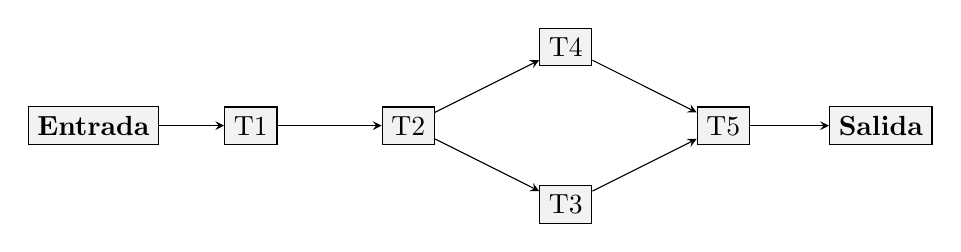
\begin{tikzpicture}[every node/.style={draw, fill=gray!10}, node distance=2cm]
            \node (entrada) [draw] {\textbf{Entrada}};
            \node (T1) [draw, right of=entrada] {T1};
            \node (T2) [draw, right of=T1] {T2};
            \node (T3) [draw, right of=T2, yshift=-1cm] {T3};
            \node (T4) [draw, right of=T2, yshift=1cm] {T4};
            \node (T5) [draw, right of=T4, yshift=-1cm] {T5};
            \node (salida) [draw, right of=T5] {\textbf{Salida}};
            
            \draw[-stealth] (entrada) -- (T1);
            \draw[-stealth] (T1) -- (T2);
            \draw[-stealth] (T2) -- (T3);
            \draw[-stealth] (T2) -- (T4);
            \draw[-stealth] (T3) -- (T5);
            \draw[-stealth] (T4) -- (T5);
            \draw[-stealth] (T5) -- (salida);
        \end{tikzpicture}
        \caption{Segmentación del Ejercicio~\ref{ej:2.9}.}
    \end{figure}
    La entrada tenemos que es el bloque de la imagen a decodificar (supone 8x8 pixels de la imagen).
    La salida será el bloque decodificado de 8x8 pixel. Las tareas 1, 2 y 5 se ejecutan en un tiempo igual a $t$,
    mientras que las tareas 3 y 4 suponen $1.5t$. El decodificador JPEG aplica el grafo de tareas de la figura a bloques de la imagen, cada uno de 8x8 píxeles. Si
    se procesa una imagen que se puede dividir en $n$ bloques de 8x8 píxeles, a cada uno de esos $n$ bloques se
    aplica el grafo de tareas de la figura. Obtenga la mayor ganancia en prestaciones que se puede conseguir
    paralelizando el decodificador JPEG en (suponga despreciable el tiempo de comunicación/sincronización):
    \begin{enumerate}
        \item 5 procesadores.
        \item 4 procesadores.
    \end{enumerate}

    En cualquier de los dos casos, la ganancia se tiene que calcular suponiendo que se procesa una imagen con un total de $n$ bloques de 8x8 píxeles.


\begin{enumerate}
    \item
    Contamos con 4 etapas en el cauce, ya que el bloque 3 y 4 se ejecutan en paralelo al poder asignar cada tarea a un procesador.
    Veamos en qué momento entra y sale de cada etapa, para ver cómo evoluciona el cauce:
    \begin{table}[H]
        \begin{tabular}{|c|c|c|c|c|c|c|c|c|}
            \hline
            Bloque & Entra 1 & Sale 1 & Entra 2 & Sale 2 & Entra 3 & Sale 3 & Entra 4 & Sale 4 \\
            \hline
            B1 & 0 & $t$ & $t$ & $2t$ & $2t$ & $3.5t$ & 3.$5t$ & 4.$5t$ \\
            B2 & $t$ & $2t$ & $2t$ & $3t$ & $3.5t$ & $5t$ & $5t$ & $6t$ \\
            B3 & $2t$ & $3t$ & $3t$ & $4t$ & $5t$ & $6.5t$ & $6.5t$ & $7.5t$\\
            B4 & $3t$ & $4t$ & $4t$ & $5t$ & $6.5t$ & $8t$ & $8t$ & $9t$\\
            \hline
        \end{tabular}
    \end{table}
    Desde que sale el bloque 1 hasta el bloque 2, transcurren $1.5t$, al igual que desde 2 hasta 3 y desde 3 hasta 4. En un cauce,
    el tiempo de ejecución depende del TLI (Tiempo de Latencia Inicial) y del TEML (Tiempo de la Etapa Más Lenta). En este caso, el TLI es $4.5t$, ya que es el tiempo que tarda en llenarse el cauce.
    El TEML es $1.5t$, que es la tercera etapa. Por tanto, el tiempo de ejecución en paralelo es:
    \begin{align*}
        T_P(5) &= \underbrace{4.5t}_{B1} + \underbrace{1.5t}_{B2} + \underbrace{1.5t}_{B3} + \cdots + \underbrace{1.5t}_{Bn}\\
        &= \text{TLI} + (n-1)\text{TEML} = 4.5t + 1.5t(n-1) = 3t + 1.5tn
    \end{align*}

    El tiempo secuencial tenemos que es:
    \begin{equation*}
        T_S(n) = n\cdot (t+t+2\cdot 1.5t+t) = 6nt
    \end{equation*}

    Por tanto, la ganancia tenemos que es:
    \begin{equation*}
        S(5,n) = \dfrac{T_S(n)}{T_P(5,n)} = \dfrac{6nt}{3t + 1.5tn} = \dfrac{6n}{3 + 1.5n}
    \end{equation*}

    La ganancia máxima se obtiene cuando $n\rightarrow\infty$, que es cuando el cauce estará lleno:
    \begin{equation*}
        \lim_{n\to\infty}S(5,n) = \lim_{n\to\infty}\dfrac{6n}{3 + 1.5n} = \dfrac{6}{1.5} = 4
    \end{equation*}

    \item En este caso, la asignación de procesadores no es trivial, pues no podemos asignar cada tarea a un procesador.
    Las tareas 3 y 4 tendrán un único procesador por ser las más lentas. Así, tenemos que:
    \begin{itemize}
        \item La tarea 1 al procesador 1.
        \item La tarea 2 al procesador 1.
        \item La tarea 3 al procesador 2.
        \item La tarea 4 al procesador 3.
        \item La tarea 5 al procesador 4.
    \end{itemize}
    Se trata de una distribución en 3 etapas para segmentación, donde la primera etapa se corresponde con las dos primeras tareas, la segunda con la tercera y la cuarta, y la tercera con la quinta.
    En este caso, tenemos que el TEML es de $2t$, y que el TLI es de $(2+1.5+1)t=4.5t$. Por tanto, el tiempo de ejecución en paralelo es:
    \begin{equation*}
        T_P(4) = 4.5t + 2t(n-1) = 4.5t + 2tn - 2t = 2tn + 2.5t
    \end{equation*}
    
    Por tanto, la ganancia en prestaciones es:
    \begin{equation*}
        S(4,n) = \dfrac{6nt}{2tn + 2.5t} = \dfrac{6n}{2n + 2.5}
    \end{equation*}

    La ganancia máxima se obtiene cuando $n\rightarrow\infty$, que es cuando el cauce estará lleno:
    \begin{equation*}
        \lim_{n\to\infty}S(4,n) = \lim_{n\to\infty}\dfrac{6n}{2n + 2.5} = \dfrac{6}{2} = 3
    \end{equation*}
\end{enumerate}


\end{ejercicio}


\begin{ejercicio}
    Se quiere implementar un programa paralelo para un multicomputador que calcule la siguiente
    expresión para cualquier $x$ (es el polinomio de interpolación de Lagrange):
    $P(x) = \sum\limits_{i=0}^{n} \left(b_i\cdot L_i(x)\right)$, donde:
    \begin{align*}
        L_i(x) &= \frac{(x-a_0) \ldots  (x-{a_{i-1}})(x-{a_{i+1}}) \ldots  (x-a_n)}{k_i}
        = \frac{\prod\limits_{\substack{j=0\\ j\neq i}}^{n} (x-a_j)}{k_i} \qquad i=0,1,\dots,n\\
        k_i &= (a_i-a_0) \ldots  (a_i-a_{i-1})(a_i-a_{i+1}) \ldots  (a_i-a_n)= \prod\limits_{\substack{j=0\\ j\neq i}}^{n} (a_i-a_j) \qquad i=0,1,\dots,n
    \end{align*}

    Inicialmente $k_i$, $a_i$ y $b_i$ se encuentran en el nodo $i$ y $x$ en todos los nodos. Sólo se van a usar funciones de
    comunicación colectivas. Indique cuál es el número mínimo de funciones colectivas que se pueden usar,
    cuáles serían, en qué orden se utilizarían y para qué se usan en cada caso.
\end{ejercicio}

\begin{ejercicio}\label{ej:2.11}~
    \begin{enumerate}
        \item Escriba un programa secuencial con notación algorítmica (podría escribirlo en C) que
        determine si un número de entrada, $x$, es primo o no. El programa imprimirá si es o no primo. Tendrá
        almacenados en un vector, \verb|NP|, los $M$ números primos entre 1 y el máximo valor que puede tener un número
        de entrada al programa.

        \item Escriba una versión paralela del programa anterior para un multicomputador usando un estilo de
        programación paralela de paso de mensajes. El proceso 0 tiene inicialmente el número $x$ y el vector \verb|NP| en su
        memoria e imprimirá en pantalla el resultado. Considere que la herramienta de programanción ofrece
        funciones \verb|send()/receive()| para implementar una comunicación uno-a-uno asíncrona, es decir, con función
        \verb|send(buffer,count,datatype,idproc,group)| no bloqueante y
        \verb|receive(buffer,count,datatype,idproc,group)| bloqueante. En las funciones \verb|send()/receive()| se
        especifica:
        \begin{itemize}
            \item \verb|group|: identificador del grupo de procesos que intervienen en la comunicación.
            \item \verb|idproc|: identificador del proceso al que se envía o del que se recibe.
            \item \verb|buffer|: dirección a partir de la cual se almacenan los datos que se envían o los datos que se
            reciben.
            \item \verb|datatype|: tipo de los datos a enviar o recibir (entero de 32 bits, entero de 64 bits, flotante de 32
            bits, flotante de 64 bits, \dots).
            \item \verb|count|: número de datos a transferir de tipo \verb|datatype|.
        \end{itemize}
    \end{enumerate}
\end{ejercicio}

\begin{ejercicio} \label{ej:2.12}
    Escribir una versión paralela del programa secuencial del ejercicio~\ref{ej:2.11} para un multicomputador
    usando un estilo de programación paralela de paso de mensajes y suponiendo que la herramienta de
    programación ofrece las funciones colectivas de difusión y reducción (escribir primero la versión secuencial). 
    Sólo el proceso 0 imprimirá en pantalla. En la función de difusión,
    \verb|broadcast(buffer,| \verb|count,datatype,| \verb|idproc,group)|, se especifica:
    \begin{itemize}
        \item \verb|group|: identificador del grupo de procesos que intervienen en la comunicación, todos los procesos
        del grupo reciben.
        \item \verb|idproc|: identificador del proceso que envía.
        \item \verb|buffer|: dirección de comienzo en memoria de los datos que difunde \verb|idproc| y que almacenará,
        en todos los procesos del grupo, los datos difundidos.
        \item \verb|datatype|: tipo de los datos a enviar/recibir (entero de 32 bits, entero de 64 bits, flotante de 32
        bits, flotante de 64 bits, \dots).
        \item \verb|count|: número de datos a transferir de tipo \verb|datatype|.
    \end{itemize}
    En la función de reducción, \verb|reduction(sendbuf,| \verb|recvbuf,count,| \verb|datatype,oper,| \verb|idproc,group)|,
    se especifica:
    \begin{itemize}
        \item \verb|group|: identificador del grupo de procesos que intervienen en la comunicación, todos los procesos
        del grupo envían.
        \item \verb|idproc|: identificador del proceso que recibe.
        \item \verb|recvbuf|: dirección en memoria a partir de la cual se almacena el escalar resultado de la reducción
        de todos los componentes de todos los vectores \verb|sendbuf|.
        \item \verb|sendbuf|: dirección en memoria a partir de la cual almacenan todos los procesos del grupo los
        datos de tipo \verb|datatype| a reducir (uno o varios).
        \item \verb|datatype|: tipo de los datos a enviar y recibir (entero de 32 bits, entero de 64 bits, flotante de 32
        bits, flotante de 64 bits, \dots).
        \item \verb|oper|: tipo de operación de reducción. Puede tomar los valores \verb|OR|, \verb|AND|, \verb|ADD|, \verb|MUL|,\verb|MIN|,\verb|MAX|
        \item \verb|count|: número de datos de tipo \verb|datatype|, del buffer \verb|sendbuffer| de cada proceso, que se van a reducir.
    \end{itemize}
\end{ejercicio}

\begin{ejercicio}~
    \begin{enumerate}
        \item\label{ej:2.13a} Escribir una versión paralela del programa paralelo del ejercicio~\ref{ej:2.12} suponiendo que, además de las
        dos funciones colectivas anteriores, se dispone de dispersión y que $M$ es divisible entre el número de
        procesos (escribir primero la versión secuencial). Sólo el proceso 0 imprimirá en pantalla. La función
        \verb|scatter(sendbuf,sendcnt,recvbuf,recvcnt,datatype,idproc,group)| especifica:
        \begin{itemize}
            \item \verb|group|: identificador del grupo de procesos que intervienen en la comunicación, todos los procesos
            del grupo envían.
            \item \verb|idproc|: identificador del proceso que envía.
            \item \verb|recvbuf|: dirección en memoria a partir de la cual se almacenan los datos recibidos.
            \item \verb|sendbuf|: dirección en memoria a partir de la cual almacena el proceso \verb|idproc| los datos a enviar.
            \item \verb|sendtype|: tipo de los datos a enviar y recibir.
            \item \verb|recvcnt|: número de datos de tipo \verb|datatype| a recibir en \verb|recvbuf|.
            \item \verb|sendcnt|: número de datos de tipo \verb|datatype| a enviar.
        \end{itemize}

        \item ¿Qué estructura de procesos/tareas implementa el código paralelo del apartado~\ref{ej:2.13a}? Justifique su respuesta.
    \end{enumerate}
\end{ejercicio}

\begin{ejercicio}
    Escribir una versión paralela del programa secuencial del ejercicio~\ref{ej:2.11} para un multiprocesador
    usando el estilo de programación paralela de variables compartidas; en particular, use OpenMP (escribir
    primero la versión secuencial).
\end{ejercicio}

\subsection{Cuestiones}
\begin{cuestion}
    Indique las diferencias entre OpenMP y MPI.\\

    OpenMP es una API de directivas y funciones, mientras que MPI es una API de funciones. Ambas son herramientas que permiten desarrollar paralelismo. Sin embargo, como hemos ya mencionado en la parte teórica, la abstracción en la que nos sitúa OpenMP es mayor a al que nos provee MPI: mientras que en MPI hemos de preocuparnos de muchos detalles a la hora de implementar el paralelismo, en OpenMP le decimos a la herramienta que realice cierta tarea y ya es el compilador quien se encarga de resolver estos detalles.
\end{cuestion}

\begin{cuestion}
    Ventajas e inconvenientes de una asignación estática de tareas a procesos/threads frente a una asignación dinámica.\\

    La principal desventaja de la asignación dinámica frente a la estática es la necesidad de calcular en cada momento qué asignación de trabajo es la mejor a desarrollar en cada momento: tener en cuenta qué nodos de trabajo se encuentran ocupados y cuales no y dividir el trabajo conforme a ello.
    Esto puede llevar a una sobrecarga de trabajo en el cálculo de la asignación de tareas, lo que puede llevar a una pérdida de tiempo en la ejecución del programa. Como ventajas, podemos destacar dos:
    \begin{itemize}
        \item En caso de una asignación compleja (podemos realizar una asignación estática, pero obtenerla es muy dificultosa), podemos simplemente realizar una asignación dinámica, ahorrando al programador la tarea del cálculo de los trabajos de cada nodo.
        \item Cuando no se conoce el número de tareas que se ejecutarán (por ejemplo, porque depende de un parámetro que se conoce en tiempo de ejecución), no es posible llevar a cabo una asociación estática.
    \end{itemize}
\end{cuestion}

\begin{cuestion}
    ¿Qué se entiende por escalabilidad lineal y por escalabilidad superlineal? Indique las causas por las que se puede obtener una escalabilidad superlineal.\\

    Decimos que un programa que resuelve una aplicación de forma paralela es escalable linealmente cuando su ganancia de velocidad en comparación con el tiempo secuencial resulta en el número de procesadores. Es decir, decimos que una aplicación paralela escala linealmente si:
    \begin{equation*}
        S(p) = p
    \end{equation*}
    Por otra parte, decimos que escala de forma superlineal si:
    \begin{equation*}
        S(p) > p
    \end{equation*}
    Un ejemplo de escalabilidad superlineal es el resultado de aplicar una búsqueda lineal paralela a cierta instancia, de forma que en pocas iteraciones encuentre el elemento buscado gracias a partir el vector para su paralelización, tal y como comentamos en la Sección~\ref{ej:superlineal}.
\end{cuestion}

\begin{cuestion}
    Enuncie la ley de Amdahl en el contexto de procesamiento paralelo.\\

    Dado un código secuencial cuyo tiempo de ejecución suponemos constante en $T_S$ segundos, suponemos que tenemos una fracción $f$ de código no paralelizable y que usamos $p$ procesadores para la fracción de código que sí es paralelizable. En dicho caso, obtendremos una ganancia con $p$ procesadores de a lo sumo:
    \begin{equation*}
        S(p) \leq \dfrac{p}{1+f(p-1)}
    \end{equation*}
\end{cuestion}

\begin{cuestion}
    Deduzca la expresión matemática que se suele utilizar para caracterizar la ley de Gustafson. Defina claramente y sin ambigüedad el punto de partida que va a utilizar para deducir esta expresión y cada una de las etiquetas que utilice. ¿Qué nos quiere decir Gustafson con esta ley?\\

    Supuesto que el tiempo de ejecución de un código paralelo es constante fijado un número $p$ de procesadores en $T_P(p)$, procedemos a calcular el tiempo de ejecución secuencial de dicho programa en función del tiempo de ejecución en paralelo, sabiendo que existe una fracción $f$ de código no paralelizable:
    \begin{equation*}
        T_S = f\cdot T_P(p) + p(1-f)\cdot T_P(p)
    \end{equation*}
    Ya que la fracción de código no paralelizable será la misma. Además, si antes tardábamos $(1-f)T_P(p)$ en ejecutar la parte paralelizable entre $p$ procesadores, si asumimos un reparto equitativo, en un procesador tendremos que hacer $p$ veces este tiempo. De esta forma, calculamos la ganancia:
    \begin{equation*}
        S(p) = \dfrac{T_S}{T_P(p)} = \dfrac{f\cdot \cancel{T_P(p)} + p(1-f)\cancel{T_P(p)}}{\cancel{T_P(p)}} = f+p(1-f)
    \end{equation*}
    Con esta ley, Gustafson nos indica que la ganancia depende de forma lineal del número $p$ de procesadores, con una pendiente de $1-f$, lo que nos indica que, a mayor sea $1-f$ (luego, menor sea $f$), es decir, la parte paralelizable; mayor será la ganancia de velocidad al paralelizar.
\end{cuestion}

\begin{cuestion}
    Deduzca la expresión que caracteriza a la ley de Amdahl. Defina claramente el punto de partida y todas las etiquetas que utilice.\\

    Supuesto que el tiempo de ejecución de un programa en un procesador es constante en $T_S$ segundos y supuesto que pasamos a una versión del programa con código paralelo con $p$ procesadores y una fracción de código no paralelizable $f$. Bajo estas hipótesis, calculamos el tiempo de ejecución en paralelo a partir del secuencial:
    \begin{equation*}
        T_P(p) = T_C(p) + T_O(p) = f\cdot T_S + \left(\dfrac{1-f}{p}\right)\cdot T_S + T_O(p)
    \end{equation*}
    Debido a que tenemos una fracción $f$ no paralelizable y que la parte que tardaba $(1-f)\cdot T_S$ se reparte de forma equitativa entre $p$ procesadores. De esta forma, calculamos la ganancia:
    \begin{equation*}
        S(p) = \dfrac{T_S}{f\cdot T_S + \left(\dfrac{1-f}{p}\cdot T_S\right) + T_O(p)} = \dfrac{1}{f + \dfrac{1-f}{p} + \dfrac{T_O(p)}{T_S}}   
    \end{equation*}
    Con $\dfrac{T_O(p)}{T_S} > 0$, luego obtendremos la mayor ganancia cuando $T_O(p)$ sea despreciable, por lo que cualquier ganancia estará limitada:
    \begin{equation*}
        S(p) \leq \dfrac{1}{f+\dfrac{1-f}{p}} = \dfrac{p}{1+f(p-1)}
    \end{equation*}
\end{cuestion}
